\section{A General Theory of Meaning}\label{sec:theory}

We present a general theory of meaning applicable across agent types (human, machine, etc.) and multimodal contexts. 
It is helpful to read this section as a genealogy of `social objects' such as moral values (fairness, liberty, equality) and social categories (race, class, gender).
%\jared{can cite hacking, looping effect}
% Citation moved as a concrete example to 'meaning in practice'
Such social objects begin, spurred on by context, inside the individual as totally abstract and become more actualized over time.
%\andre{do you also want to mention the context? not just individual $\to$ world, but also world $\to$ individual}
As they become more concrete, they eventually enter into the shared social-material world, altering what was already there.
In a full circle, our social constructions begin to have material effects, which become new contexts that ground concretization.
``Social kinds'' are one prominent example of this ``looping effect'' \citep{Hacking:LoopingEffects}.
%, such as autism, disability, depression, and multiple-personality disorder.
% insofar as they regulate people, coming to change the way in which people mean.

This theory does not aim to describe its own `implementation' in meaning-agents. 
Instead, this theory provides an efficacious model for discussing the many similarities between meaning-agents.
% under a unified language.

%\markC{Possibly delete, not really necessary}
%As a methodological note, it is helpful to view many of the concepts in this paper as following binary structures that proceed from abstract to concrete. This general form is useful for framing many dichotomies in both the semiotic and ethical realms. A small list follows: Abstract $\to$ Concrete, Sign $\to$ Object, Concept $\to$ Context, Internal $\to$ External, Reification $\to$ Inscription, Concept $\to$ Content.

\begin{table}[!ht]
\centering
\begin{tabular}{l|l}
\toprule
Term            & Brief Description \\
\midrule
%Phenomenon      & A basic and independent unit of experience \\
Signification   & A relationship between two experiences, one of which picks out the other. \\
Context         & A material/social arrangement which imposes structure upon experience. \\
Sign            & An experience taken as signifying another experience. \\
Object          & An experience taken as being signified by another experience. \\
Concept         & An internalization of a context, regulating a set of sign-object relationships. \\
Determination   & The process of an object acquiring a signification. \\
Concretization  & A process of individual objects being determined by the context. \\
Inscription     & A process of altering the context through the exercise of concepts. \\
Social Totality  & The social arrangement governing a community of people. \\
\bottomrule
\end{tabular}
\jared{Do we just mean people here or could the social totality refer also to a community of models e.g. in the recent alpaca farm paper?}
\end{table}

\subsection{Snapshots of meaning}

We will begin by discussing how our general theory of meaning operates at snapshots in time.
First, we start with pure individual experience in the snapshot before meanings emerge.
% We should immediately note something which will inevitably be found strange about the way we discuss experiences.
Importantly, according to our model of experience, all experiences begin by grasping a `thisness' of something \citep{Hegel:PhG}.
For example, suppose there is a table in a room.
The table might be brown, mottled with age, stained with food, etc.
This table has a variety of properties.
But an individual, upon first seeing the table, does not stop to pay attention to its brownness, its age, its uncleanliness, and so on.
Instead, this individual merely grasps that this table is a thing -- the `thisness' of the table.
If the individual has never seen a table before, they might not even grasp that it is in fact a table.
The individual's experience of the table is thus \textit{surprisingly empty}.
This experience has no internal contents or particularities, it just \textit{is}.
Because of this, we say that \textit{experiences begin as }\textbf{abstract}.
This initial abstractness of the experience allows us to avoid the pitfalls of qualia (ineffable, intrinsic, immediate, private \citep{Dennett:QuiningQualia} subjective experiences such as the redness of an apple).
\jared{I like this example. Very solid.}

Over time, experiences become interrelated; they fall into certain roles with respect to one another.
Now, we will consider a snapshot wherein meanings have begun to develop -- that is, experiences have become related.
We call a relation between experiences a \textbf{signification}.
With a signification, one experience picks out another experience for an agent.
We call the experience that does the picking out the \textbf{sign}.
The experience being picked out is the \textbf{object} of that sign.
This description applies to all relations between experiences for any agent.
For an animal, a loud noise signifies a potential threat.
For humans using language, a name signifies a person.
The way in which the loud noise signifies the threat is very different from the way in which a name signifies a person.
The former does so through an automatic physiological response, the latter does so through language.
This `way of signifying' is the result of an external arrangement, social or material, imposing itself on experience.
For the animal, this arrangement is its evolutionary biology.
For a human using language, this arrangement is the language-game (a set of conventions that regulate the usage of language in a certain context \citep{Wittgenstein:PhilosophicalInvestigations}). 
This external arrangement is the \textbf{context}.
We might implicitly internalize the context (perhaps by learning the rules of the language-game over time).
A way of internalizing a context with respect to a set of meanings is a \textbf{concept}.
Over time, concepts enable individuals to develop more significations.
Thus, the central maxim of our theory is ``The \textbf{concept} makes possible the \textbf{signification} of the \textbf{object} by the \textbf{sign}.''
This schema is simple but robust.
Nevertheless, there are nuances we should explore.

%\andre{what if we just introduced each term after ``we posit a triad of sign concept object''} It behooves us to explore each term further:

\begin{figure}
    \centering
    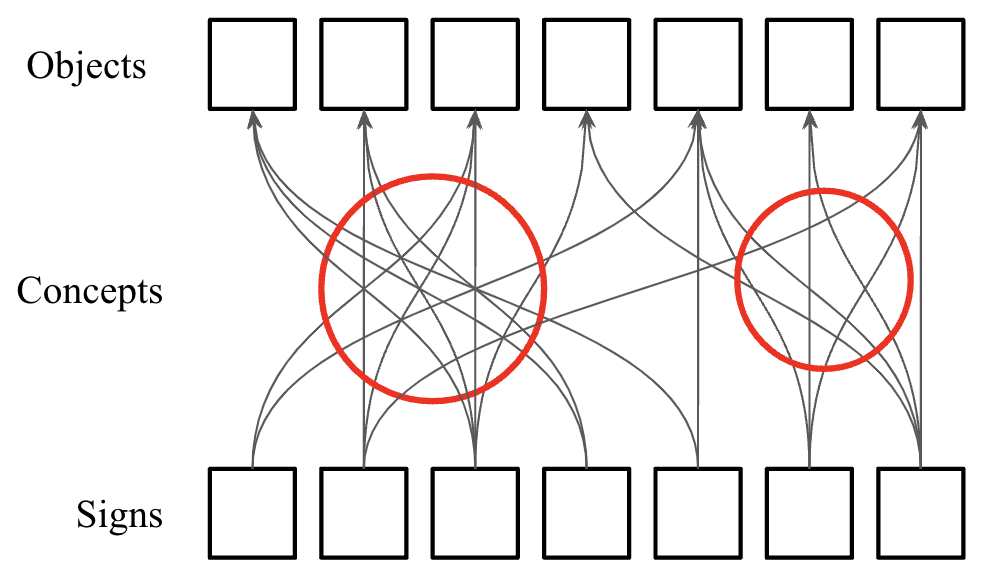
\includegraphics[width=6cm]{NeurIPS/imgs/sign-concept-object.png}
    \caption{Signification relations between \textit{signs} and \textit{objects}. Both signs and objects are empty experiences. They have no internal content, but are merely determined by their relations. Groups of significations are called \textit{concepts}.}
    \label{fig:enter-label}
\end{figure}

Recall that objects and signs are both just experiences. This allows us to explain meaning using only two sorts: \textit{experiences} and \textit{the relationships between experiences} (significations).
\footnote{This two-sortedness bears a certain similarity to category theory with its notions of objects and morphisms. This is no accident \citep{Tsuchiya:CategoryTheoryNeuroscience}.
% Category theory determines objects wholly by their morphisms. It refuses to pry open the black box of what the object is. As will soon become clear, this external determination is the central paradigm of our theory of meaning.
}
This allows us to avoid complications with objects that do not exist in the material world.
Fictional characters are a classic example -- what does a name like ``Hamlet'' refer to? For our theory, it is the experiences signified by ``Hamlet.''
\jared{I like this but possibly could cut from here to the end of the paragraph and keep the kripke citation}
Perhaps the reader has constructed an impression of Hamlet in their mind.
Perhaps the reader has seen a live performance of Hamlet and cannot get around `seeing' Hamlet as whoever played him. Each of these experiences is a potential object of the sign ``Hamlet.''
We also avoid problems with the referents of proper names (whether proper names have descriptions or whether they refer only to their real objects) by obviating the question of `real' referents entirely \citep{Kripke:NamingNecessity}.

%\markC{Graveyard of theories of meaning}
% \markC{Lose the qualia discussion as a whole, but name the problem}
% Our theory also avoids problems of qualia (ineffable, intrinsic, immediate, private \citep{Dennett:QuiningQualia} subjective experiences such as the redness of an apple).
% By speaking solely in terms of experiences and the relations between them (their significations), we never need to discuss the internal contents of experience at all.
% Instead, objects are externally determined by their relations with signs -- signs determine what objects `are.'
% Wittgenstein proposes a thought experiment: a man claims he has a beetle in a box, but can never show this beetle to the world.
% For all we know, this beetle could be anything, or in fact nothing.
% The thing in the box, whatever it may be, has no place in communication \citep{Wittgenstein:PhilosophicalInvestigations}.
% This thing in in the box is the quale, the internal content of an experience.
% In fact, qualia are not sufficient grounds of meaning, even if they may exist (a question which we need not answer).
% Moreover, because objects are externally determined by their significations, they are constantly changing as we acquire new significations. 
% Objects are \textit{dynamic}, constituted by experiential motions \citep{Lonergan:CognitionalStructure}.
% We will later expound upon this theme, the dynamism of objects, will forms a core part of our theory.

%\markC{Similarly, cut this into a simple reference}
%Finally, this two-sorted theory avoids the problems of proper names (whether proper names have descriptions or whether they refer only to their real objects). Direct referentialists posit that each proper name must have one and only one real object \citep{Kripke:NamingNecessity}. If proper names had multiple objects, it would be impossible to say anything meaningful with the name alone and no description. For example, a question about a person whom one does not know -- ``who is Nancy Reagan?'' -- proves meaningless. However, if objects are just experiences, a name alone signifies an experience of having heard that name before. Any experience can sign for multiple objects. Moreover, objects can serve as signs for other experiences.

%\markC{Chop into one sentence for later}
%So far, we have exposited a theory of two sorts: experiences and relations between experiences. These two sorts don many cloaks. We have seen experiences appear as signs and objects; we have seen relations appear as significations and concepts. These four roles account for a statics of meaning. They answer the question of how the individual, at a single moment in time, interprets an experience.

%The \textbf{object} is an object \textit{in experience}.\footnote{I.e., a `phenomenal' object.}
%An immediate concern for theories of meaning that identify objects as objects-in-the-world is how to understand signs that seemingly have no worldly objects.
%When we say `Hamlet,' we mean the character as a being in his world. 
%But by restricting us to the domain of real objects, we are forced to mean `Hamlet' as a play, a Shakespearean invention, and so on. Accordingly, we restrict the domain of reference to objects \textit{in experience}.
%\andre{I feel like this could be rewritten more clearly to get the basic point -- I can have a stab at this if you want}
%This allows us to promote a notion of dynamic objects. Objects are constantly being constituted by experiential motions; they are constantly being determined against themselves and other objects. As we will later see, this dynamism forms a core part of our theory.

%The \textbf{sign} is a function that any object may take on in relation to any other object. Insofar as an object $A$ `picks out' another object $B$ in a certain context, $A$ signifies $B$. It is quite possible for a sign to signify multiple objects \textit{in general} -- context is required to reduce the number of referents to one.
%\andre{are signs functions or also `objects' in experience? do we want to mention object and sign are of the same substance (phenomenality)?}

\subsection{A genealogy of the object}
So far, our theory of meaning has provided the grounds for understanding how meaning operates at a single snapshot in time through four roles: the concept, the sign, the signification, and the object.
We now turn to the ways in which meaning applies itself over time to produce the object (i.e., its genealogy). 
Recall that we described experiences as initially abstract. 
Now, as experiences take shape as the objects of signs (and by signing for objects), they slowly become \textbf{concrete}. 
The pure `thisness' which the experience is replaced by a rich concept, full of links to other experiences. 
Eventually, this concrete object enters the social-material world, thereby becoming fully concrete. 
These two processes are appropriately called \textbf{concretization} and \textbf{inscription}. 
Concretization is the process whereby an object becomes more concrete through acquiring significations. 
Each acquisition of a signification is called a \textbf{determination}. 
This allows us to speak of concrete objects as being more determined than abstract objects.
%\jared{as in no underdetermination at least for the meaning agent?}
Inscription is the process whereby an individual's meanings enter  the social-material world. 
This is a process of realizing the object, actualizing what before only ever existed as an experience.

\jared{there's something afoot in this section wrt who "we" are. I think you mean at times "we" as a society with pretheoretic notions of concept. but at other times in the paper you mean "we" as the authors of this paper.}
\paragraph{Concretization}
% To begin with concretization, we must first understand the concept.
Our original usage of the term `concept' to mean an internalized context may seem strange. We generally think about a concept as an idea, something we have direct access to. Usually, this idea is thought of as having (or being) content. However, these two notions prove to be the same. First, we will understand how the colloquial notion appears in our theory. We do not discuss the \textit{internal} content of experiences, so experiences must instead acquire content by determination. This \textit{external} content is their concept. This comports with the colloquial sense of `concept': the concept of an experience is the things it signifies and the things that signify it. The concept of fairness is all things fairness means and all things that mean fairness. Fairness is what it is because it is (in part) impartiality and (in part) a standard by which to measure behavior (among other significations). The concept of fairness is described by an enumeration of its significations.

% Now, we must show that this definition (a concept is all the significations of an experience) aligns with the initial definition (a concept is an internalized context). 

This definition of the concept (all the significations of an experience) aligns with our first definition of the concept (a way of internalizing a context).
Because a context is an external arrangement, it has a structure of `real' social or material objects and the relations between them \citep{Millikan:BeyondConcepts}. When these objects are experienced by us, we attempt to replicate this structure. The result of this replication is in fact the set of significations of experiences (our previous definition of concept).

%The \textbf{concept} is a set of significations. Every sign-object pair has an associated concept. Moreover, by virtue of grouping the totality of significations associated to an object together, we may speak of a unitary `concept of the object.' 
%\jared{Whose significations? Those of a particular agent/system? I'm asking: unitary with respect to what? That is a question underlying this whole $\S$: who/what is the subject of the meaning?}
%Concepts allow for the interpretation of an object \textit{as a sign} for another object. In other words, \textit{concepts ground the possibility of signification}. The most immediate example comes from the form of signs. The interpretation of words as signs for objects is made possible by the concept of language. The same is true of all other forms of representation, especially symbolic forms. At this locus of possibility, all our relevant concepts enter here in grounding the possibility of a sign representing an object.

%\jared{For particularly abstract claims like below sometimes I like to lead with the example and then abstract, but it is up to you.} \andre{+1 this would be more helpful}
%From this functional definition, it follows that every concept is also a context of interpretation, which is most useful in understanding such abstract concepts as time (or a specific time) insofar as they contextualize and make possible the interpretation of an object as a sign for another object. This context of interpretation is also the same context required to disambiguate between multiple objects of a particular sign. Two examples serve -- a) names may differ in meaning across temporal contexts (i.e. as associated with the concept of a certain time: yesterday, today, tomorrow); b) symbols may differ in meaning across formal contexts (i.e. as representing pictorially, linguistically, etc.).

%Having introduced the triadic model, we shall study the two ways in which the triadic structure operates over time \andre{or how about just ``how meaning emerges and changes over time''}. The first, \textbf{reification}, consists in the creation and adjustment of concepts. The second, \textbf{inscription} consists in putting meanings back into the world by taking actions.

%`Reification' may seem strange to use in describing this principle of conceptual modification, but an analysis of its operation will show that `reification' is very precise as a term. Reification is generally defined as a concretization of an idea; its passage from abstract into concrete over time. In our usage, reification is the reification of objects -- the passage of objects from being purely abstract to being totally concrete. This reification occurs through determination: over time, an object is determined against itself and other objects by some relations. This perspective of determination is a new lens (beyond relation, association, and signification)
%\jared{I see we have discussed signification but have we discussed relation and association?}
%whereby to view concepts. Insofar as a concept is the signifying of an object by a sign, it is also the determining of that object by the sign and the sign (as object) by the object.

Because concretization is a process of determination (acquiring significations), both the creation and adjustment of concepts are processes of concretization. Operationally, creation and adjustment differ heavily. Efficacious creation of a concept requires that the meaning-agent clearly prioritize a context. Once this prioritization is done, the actual creation follows as something simple. For example, the context ``the English language-game'' is prioritized
\footnote{We anticipate the rejoinder that this prioritization is where we have hidden intentionality; this may well be true. We highlight this as an area for further development. However, we should note that by sequestering intentionality within prioritization, we have made a link between intentionality and unitarity (see $\S$ \ref{sec:moral}) while allowing non-intentional systems of meaning to mean in non-unitary ways.
\jared{Try to shorten this to two lines.}
}
; a word such as `table' is determined against an object, a `real' table (potentially) in the world, therefore becoming concretized.
%\jared{Is it reallyt that clean? It seems to me that there is a lot of work that goes into even knowing that "table" when said aloud is meant to signify for an object. Even then, there is Quine's point from Word and Ojbect about underdetermination---don't we immediately need to adjust our concepts to forestall against misinterpretation? Maybe it is clean when you are an established language user?}
However, a failure to adequately prioritize a context can result in scattered, non-efficacious concepts.
Adjustment, however, occurs under a predetermined context. If `table' is made to refer to all tables instead of just a singular table in the world, the original determination continues to exist under a different context.
%In this way, error consists in a re-prioritization between different contexts wherein determinations for the same object obtain, usually temporal contexts. Since contexts become internalized as concepts, we must be clear here: contexts themselves do not change here and are only prioritized or deprioritized; the determinations within them acquire priority by virtue of the priority of their context.

%\jared{and we're not trying to say how those priorities work, right?}
%\andre{another idea: error can maybe be another $\S$ after reifiction / inscription --- doesnt seem essential to reification so much as a neat application}

%\markC{Inscription is not as simple as putting what is in your head into the world - chop out the Quine references, ditch the Lonergan, move from the problem to the axiom}

\paragraph{Inscription}
Broadly speaking, inscription is the process of writing objects into the world. \textit{However, inscription is not as simple as a direct transfer from the experiential world to the social-material world}. This may seem problematic -- after all, this process is the one on which all communication depends. However, since communication is possible, we can infer that inscription must work in a certain way (approximately speaking).

\jared{I might cut this paragraph and then put the quine citation on the first sentence of the next paragraph}
One common paradigm in linguistics and semiotics is that meaning consists in reference to real (social or material) objects. If two subjects communicating are not referring to the same real object by the same term, they do not mean the same thing. As an example, this assumption grounds the theoretical impossibility of translation \citep{Quine:WordObject}. Two subjects using different languages have different sets of referents. We claim that even subjects using the same language have different sets of referents.

So, for meaning to be possible, we posit that meaning can in fact function when the referents of terms in a language are underdetermined. In fact, \textit{meaning is always underdetermined}. Because objects are externally determined, communicators are always referring to any number of potential social or material objects. Meaning happens when relations between these social or material objects correspond to relations between experiential correlates (of these social or material objects) for both communicators. This correspondence is precisely what inscription must then produce. We claim, then, that \textit{in a vacuum (with no other social or material forces), inscription by a meaning-agent produces social or material objects with determinations that correspond to the determinations of experience for that meaning-agent}. This is our ``postulate of inscription.''

\jared{these are no longer external, "social or material" objects but are rather internal experiential objects, right? Need some clarification here or above}
\jared{Maybe part of my problem is not being clear on what you mean by 'social-material'}
Objects, once inscribed, are now at their most concrete. All possible properties (e.g. location, time, composition) are determined. Some of these determinations happen arbitrarily because they have no correlate in the mind. For example, the chemical makeup of the paint in a painting is usually not determined for the painter.

This gives us \textit{a genealogy of the object}: the object begins in the experiential world as totally abstract, an undetermined `thisness'. Over time, it accrues determinations, becoming gradually more concrete. Eventually, it proceeds out into the social-material world, where it is at its most concrete. This procession redetermines the structures of the social-material world, creating a cyclic effect whereby inscription by agents conditions future concretization.

%Inscription deceives us with its seeming simplicity. 
%\andre{italicizing relevant terms and new keywords would be helpful} 
%Its name evokes its primary instance, writing, and it seems (in theory) clear enough. One has ideas, one has meanings, now one merely acts on them; meanings are inscribed into the world. But this simple gloss belies the ethical and metaphysical complexity of the act. In lieu of this complex discussion, we instead pose an open question for ethics: can agents act contrary to what they know to be absolutely and incontrovertibly true (both positively and normatively) -- in ways radically unintelligible to reason? If agents can, inscription poses a problem: our internal structures may never make it into the real world to be meant. In fact, there is very good evidence to suggest that agents can act in seemingly unintelligible ways -- any child who has ever been told to do something they know well is good for them must experience this.
%\jared{ha well said but oh so abstract. let's add an example}

%This notion of radical unintelligibility \citep{Lonergan:Insight} seems to pose serious problems for our theory. In fact, it jeopardizes the whole possibility of communication. In \textit{Word and Object}, Quine articulates a radical indeterminacy of translation caused by the lack of shared realms of material meaning between cultures \citep{Quine:WordObject}. If we believe for even a second in the possibility of radical unintelligibility, Quine's argument risks applying to all human communication, since no individual would ever have a determinately shared realm of material meaning with another.

%However, humans communicate -- it happens, and this is not a controversial assumption. Humans communicate in the absence of shared realms of material meaning too -- translation may be theoretically impossible, but it happens practically every day. We may make two moves to explain this fact. First, humans don't require shared realms of material meaning to communicate. All that they require is a material realm that possesses enough structural similarity. 

%Second, in order to facilitate this, we posit \andre{hypothesize makes it sound empirical -- I think we can just say ``claim'' right?} -- without providing a specific mechanism of inscription -- that inscription naturally produces groups of real objects equivalent (in a vacuum, considering no other material factors) to the same groups of phenomenal objects according to the relations between them. It is this equivalence of inscription that makes meanings meaningful, under this system. Agents inscribe equivalent categories into the material world, whereupon other agents, in reifying for themselves a set of efficacious associations, will naturally recover equivalent categories internally.

%\jared{Where do we stand on isomorphism vs equivalence? Did we decide isomorphism?}

%\markC{Cut this up, lose the infinite iterability}
%The final difficulty with inscription is that communication does not always happen. Therefore, for our notion of inscription to be cogent, we must be precise and incorporate potentiality: inscription is the production of equivalent structures in the material world by an agent which could \textit{potentially} be recovered by (other) agents. This potentiality is a ground of infinite iterability; inscription ensures that the inscribed lives on long past the author. The inscribed objects lose their privacy, their internal content; they are understood as externally determined.
%This is how we respond to the nonsensicality of the private language \citep{Wittgenstein:PhilosophicalInvestigations}. In this sense, inscription is another kind of concretization in the colloquial sense -- an idea, once merely abstract, becomes concrete as it is put out into the world.
%\andre{like this description a lot}

%We are finally equipped to describe the genealogy of an object: an object begins as an undetermined, nebulous mass in the phenomenal world. It quickly acquires a singular, cardinal determination (the moment of creation) and thereafter continues to be determined across different contexts. Ultimately, its determinations are reproduced at the moment of its inscription into the material world.

%\jared{substrate of materiality seems like a term that should be put in the box. also not sure how approachable it is}


\subsection{The social object}\label{sec:theory:social}
This theory of meaning also gives us the appropriate tools to describe the object as it passes beyond the experiential world and into the social (material) world -- in other words, the object as a \textbf{social object}. This discussion of the social object will prefigure our forthcoming analysis of values and categories insofar as they are themselves social objects -- most pertinently, for example, morality.
%, but also gender, race, class, etc.

Recall our ``postulate of inscription'': in a vacuum, inscription reproduces the determinations of the object it inscribes.
%Under this assumption, material objects can continue to have internal contents which may or may not be perceptible, but remain structurally perceptible via their external determinations.\footnote{This idea of a material structure of objects is broadly similar to the ontology of right-wing Sellarsians (i.e. Milikan).}
Now, consider a material object. It has a variety of determinations -- color, location, composition, and so on. Only some of these are ever experienced by individuals. The sum of these experiences determines a \textit{social} object. In general, a social object is a sum of determinations over individuals in a society. It is reasonable to ask in what sense the social object `really' exists. Who is the social object an object for? We claim that it is useful to posit an abstract model of society as a meaning-agent. We can treat this abstraction very much like we treat individuals. It has its own concepts, signs, significations, and objects. We do not have to be ontologically committed to its existence for it to be very useful. Generally speaking, this abstraction is something like our collective ground of meaning as a society.

We give this abstraction the name \textbf{social totality}, emphasizing its nature as a system of meaning. Then, \textit{the objects of the social totality are the social objects.} \textit{Moreover, the }\textbf{concepts}\textit{ of the social totality are many of the }\textbf{contexts}\textit{ about which we have been writing.} For example, the language-game, which operates as as \textit{context} for an individual, is a \textit{concept} for the social totality \citep{Gadamer:TruthAndMethod, Heidegger:BeingAndTime}. \textit{In fact, all social contexts are concepts of the social totality.} This means that the social totality accrues a variety of concepts in which to determine objects.

% This social totality is an abstraction -- we do not need to be ontologically committed to its existence -- but it is useful insofar as it allows us to analogize between our own common ground of meaning and ourselves as experiencing beings. 
% Although we do not need to be ontologically committed to it, the concept of social totality and our own ground of experience have the same structure of meaning.
%Both our individual and collective grounds of meaning (the latter being the ``social totality'') have the same structure: that of sign, concept, and object.
%Under this structure, the social totality has as its \textit{objects} precisely these social objects in abstract.
%Its \textit{determinations} are the determinations which we inscribe into its corpus (in a literal and textual sense). 
%Its objects are \textit{determined} by those individual significations which we inscribe into the corpus of the social totality. 
%\jared{How is this inscription occurring?}
%Its internal concepts are in fact what we have called contexts; contexts are the concepts of the social totality.

Because of this diversity of concepts, when considered as a meaning-agent, the meanings of the social totality are highly indeterminate. Thus, the social totality is perpetually in conflict with itself. This constant struggle is the social history of the object~\citep{foucault2002order}. In a certain sense, then, the truth of social totality is eternal self-contradiction~\citep{Hegel:PhG}. But it is a powerful kind of self-contradiction comprised by multitudes of information grouped according to their contexts. So we must be precise: to understand the kind of contradiction involved in any concept, we must understand the concepts which compose it, the histories, peoples, and diverse points of view which go into making a concept what it is. 

Let us now consider an example in practice -- how does a child learn what `fairness' means? `Fairness' begins as a social structure -- a \textit{social object} for the \textit{social totality}. A child learns certain things from their society about norms of behavior and judgment. They begin to relate instinctual \textit{experiences} of being wronged to fairness. Slowly, they develop a \textit{concept} of effort as \textit{signifying} reward, or ``fair'' compensation \citep{Rawls:TheoryJustice}. These concepts -- the norms, deservingness, etc. -- over time amalgamate around the word `fairness' as it is \textit{concretized}. When this child says, ``That's unfair!'', they are doing more than pointing out some behavior that violates the norms. They are also invoking deservingness, judgement, equality, and the many other concepts with which `fairness' is related. Finally, the way this child, perhaps now grown into an adult, will write (and more broadly, act) will be reflective of the myriad ways in which they perceive ``fairness'' as an aggregate of many experiences. The potential misconceptions or priorities this person has when conceiving of fairness will go back into the world -- they will be \textit{inscribed}.

%\subsection{Meaning in practice}

%This $\S$ will be a gloss of the meaning-theory in practice which covers a single instance of `what meaning is' accounting for communication, reification, etc.

%\andre{Would be nice to have a small sentence at the bottom here just saying something like ``meaning is ...'' -- maybe like ``the interplay between sign, object, and concept. For example, the meaning of ``pass the salt please'' is the interplay between how it appears in my phenomenal experience, the conceptual intermdiary it signs trhough, and the object of the signing (an action impelled).''}
